\documentclass[11pt]{article}

\usepackage{pablo}
\usepackage{multicol}
\usepackage[a5paper,margin=1.8cm]{geometry}
\pagestyle{empty}

\begin{document}

\begin{center}
  \textsc{Devoir} --- Trinômes
\end{center}
\hrule

\begin{exercice}[Fonction carrée --- 3 points]~
  \begin{enumerate}
    \item Calculer les valeurs exactes des carrés des nombres suivants :
      $-3$ ;
      $3\sqrt2$.
    \item Ordonner, sans les calculer, les couples de nombres suivants :
      $(-1728)^2$ et $(-1729)^2$ ;
      $(\frac{1}{3})^2$ et $(0,3)^2$.
  \end{enumerate}
\end{exercice}

\begin{exercice}[Fonctions --- 4 points]On a tracé dans le graphique suivant les courbes représentatives des fonctions $f$ et $g$ définies sur $\mathbb R$ par $f(x)=x^3+2x^2-x+2$ et $g(x)=x^3-x^2-2x+1$. On admet qu'elles n'ont pas de points d'intersection.

  La question que l'on se pose est : quelle est l'abscisse $x$ de la  plus petite distance $d(x)$ entre deux points des deux courbes à la verticale l'un de l'autre ?

  \begin{center}
    \begin{tikzpicture}
      \draw[->] (-3,0) -- (4.2,0);
      \draw[->] (0,-1) -- (0,4.2);
      \draw (0,0) node[below left]{$O$};
      \draw (1,0) node{$|$} node[below]{1};
      \draw (0,1) node{$-$} node[left]{1};
      \draw[domain=-2.7:1,smooth,variable=\x,red]  plot ({\x},{\x*\x*\x+2*\x*\x-\x+2});
      \draw[domain=-1.4:2.3,smooth,variable=\x,red]  plot ({\x},{\x*\x*\x-\x*\x-2*\x+1});
      \draw[<->] (-1,1) -- (-1,4) node[midway,left]{$d$};
      \draw (-2.5,1.38) node[left]{$\mathcal{C}_f$};
      \draw (2,1) node[left]{$\mathcal{C}_g$};
    \end{tikzpicture}
  \end{center}

  \begin{enumerate}
    \item Montrer que la distance $d$ peut s'exprimer par $d(x)=3x^2+x+1$.
    \item Déterminer l'abscisse de l'extremum de $d$.
    \item Cet extremum est-il un maximum ou un minimum ?
    \item En quelle abscisse la distance verticale entre les courbes de $f$ et $g$ est-elle minimale ?
  \end{enumerate}
\end{exercice}

\hfill\emph{Tourner la page.}
\newpage

\begin{exercice}[Forme canonique --- 7 points]
  On étudie la fonction $f$ définie sur $\mathbb{R}$ par $f(x)=0,5x^2+2x-3$.
  \begin{enumerate}
    \item Montrer que $0,5(x+2)^2-5=0,5x^2+2x-3$.
    \item\label{racines} En déduire les solutions de $f(x)=0$.
    \item\label{extremum} Déterminer les coordonnées de l'extremum de $f$.
    \item Tracer la fonction $f$ dans un repère orthonormé. On prendra comme échelle (au choix) : une unité = un carreau \emph{ou} une unité = un centimètre. Le graphique ira de -7 à 3 en abscisse, et de -6 à 6 en ordonnée.
    \item Vérifier les résultats des questions \ref{racines} et \ref{extremum} sur le graphique.
  \end{enumerate}
\end{exercice}

\begin{exercice}[Problème --- 6 points]~

  \begin{multicols}{2}

    Le conseil municipal d'une commune souhaite aménager un parc carré comme sur le schéma de droite (les longueurs sont données en mètres). Les parties grisées (quatre carrés identiques) sont des fleurs ; les parties blanches représentent la pelouse.

    \columnbreak

    \begin{center}
      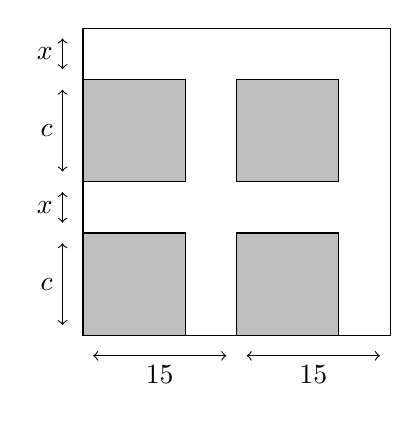
\begin{tikzpicture}[scale=0.13]
        \draw (0,0) -- ++(30,0) -- ++(0,30) -- ++(-30, 0) -- cycle;
        \foreach \i in {0, 1} {
          \foreach \j in {0, 1} {
            \draw[fill=lightgray] ({15*\i},{15*\j}) -- ++(0, 10) -- ++(10,0) -- ++(0,-10) -- cycle;
          }
        }
        \draw[<->] (1,-2) -- +(13,0) node[midway,below]{15};
        \draw[<->] (16,-2) -- +(13,0) node[midway,below]{15};
        \draw[<->] (-2,1) -- ++(0,8) node[midway,left]{$c$};
        \draw[<->] (-2,11) -- ++(0,3) node[midway,left]{$x$};
        \draw[<->] (-2,16) -- ++(0,8) node[midway,left]{$c$};
        \draw[<->] (-2,26) -- ++(0,3) node[midway,left]{$x$};
      \end{tikzpicture}
    \end{center}

  \end{multicols}

    On appelle $c$ le côté des carrés, et $x$ la largeur des allées de pelouse (verticales comme horizontales).

  La contrainte est que la pelouse doit couvrir exactement la moitié du parc. En charge de cet aménagement, vous devez déterminer les longueurs $x$ et $c$.

  \begin{enumerate}
    \item Montrer que l'aire de chaque carré grisé est donné par la formule $\mathcal{A}_c=(15-x)^2$.
    \item Montrer que $x$ vérifie $4(15-x)^2=450$.
    \item Résoudre l'équation précédente.
    \item Répondre à la question initiale : quelles doivent être la largeur $x$ des allées et le côté $c$ des carrés ?
  \end{enumerate}
\end{exercice}


\end{document}

